\documentclass[11pt]{article}

\usepackage[T1]{fontenc}
\usepackage{geometry}
\usepackage{amsmath, amssymb, amsthm}
\usepackage{listings}
% \usepackage{courier}
\usepackage{xcolor}
\usepackage{graphicx}
\usepackage{fancyhdr}
\usepackage{lipsum}
% \usepackage{subfigure}
\usepackage{caption}
\usepackage{subcaption}
\usepackage{float}
\usepackage{bm}

\newcommand\norm[1]{\| #1 \|}
\newcommand\bvec[1]{\boldsymbol{#1}}
\newcommand\kk{\bvec{k}}
\newcommand\x{\bvec{x}}
\newcommand\G{\bvec{G}}
\newcommand\ahat{\bvec{\hat{a}}}
\newcommand\bhat{\bvec{\hat{b}}}

\makeatletter
\renewcommand\@biblabel[1]{}
\renewenvironment{thebibliography}[1]
     {\section*{\refname}%
      \@mkboth{\MakeUppercase\refname}{\MakeUppercase\refname}%
      \list{}%
           {\leftmargin0pt
            \@openbib@code
            \usecounter{enumiv}}%
      \sloppy
      \clubpenalty4000
      \@clubpenalty \clubpenalty
      \widowpenalty4000%
      \sfcode`\.\@m}
     {\def\@noitemerr
       {\@latex@warning{Empty `thebibliography' environment}}%
      \endlist}
\makeatother

\captionsetup[table]{skip=10pt}

\geometry{a4paper, margin=1in, headheight=14pt}

\pagestyle{fancy}
\renewcommand\headrulewidth{0.4pt}
\fancyhead[L]{\scshape Experiment II}
% \lhead{Experiment I}
\rhead{}
\cfoot{\thepage}

\definecolor{darkgreen}{rgb}{0.2, 0.6, 0.4}
\definecolor{darkblue}{rgb}{0.2, 0.4, 0.8}
\lstset{ 
  basicstyle=\footnotesize\ttfamily,
  commentstyle=\color{gray},
  % extendedchars=true,
  % keepspaces=true,
  keywordstyle=\color{darkblue},
  % numbers=left,
  % numbersep=5pt,
  % numberstyle=\tiny\color{gray},
  stringstyle=\color{darkgreen},
  tabsize=4,
  % frame=lines,
  aboveskip=2em,
  belowskip=2em
}

\newcommand\pp[2]{\frac{\partial #1}{\partial #2}}

\title{
        \Large\textsc{PH2103: Physics Laboratory III} \\
        \vspace{10pt}
        \Huge \textbf{Wave particle duality} \\
        \vspace{5pt}
        \large{Debye-Scherrer diffraction of electrons.}
}
\author{
        \large Satvik Saha%
        \thanks{Email: \tt ss19ms154@iiserkol.ac.in}
        \\\textsc{\small 19MS154}
}
\date{\normalsize
        \textit{Indian Institute of Science Education and Research, Kolkata, \\
        Mohanpur, West Bengal, 741246, India.} \\
        \vspace{10pt}
        \today
}

\begin{document}
        \maketitle

        % \renewcommand{\abstractname}{Aims}
        \begin{abstract}
                In this experiment, we explore the phenomenon of wave particle duality via electron diffraction.
                We determine the wavelength of electrons, verify de Broglie's equation, and use this information to determine
                the lattice plane spacing of graphite.
        \end{abstract}
        
        \section{Theory}
        Wave particle duality is a a central concept of quantum mechanics. Entities such as light were long regarded as waves, since they exhibit
        phenomena such as interference and diffraction which can only be explained by a wave nature, yet other phenomena such as
        the photoelectric effect demand a quantization in terms of energy. Thus, light can also be described in terms of discrete packets of
        energy, i.e.\ photons. In a similar manner, it was thought that all matter could be described purely in terms of the particulate behaviour
        of their constituent fundamental particles, such as protons and electrons. However, it was conjectured by Louis de Broglie that
        matter also has additional wave properties, and this was confirmed by Davisson and Germer when they showed that electrons
        exhibit the phenomenon of diffraction, using crystalline nickel structures.
        The de Broglie wavelength $\lambda$ of a particle is given by 
        \[
                \lambda = \frac{h}{p},
        \]
        where $p$ is its momentum and $h$ is Planck's constant.

        \paragraph{Laue equations}
        Suppose this electron wave strikes a one dimensional crystalline lattice, where all atoms are located at positions
        $\x = a\ahat$. Here, $\ahat$ is the basis vector for the lattice. This lattice acts like a diffraction grating.
        Let the incident and scattered wavevectors be $\kk_{in}$ and $\kk_{out}$.
        
        \begin{figure}[H]
        \centering
        \includegraphics[scale=1.0]{./laue.eps}
        \caption{Scattering of a wave at a crystal plane.}
        \label{fig:laue}
        \end{figure}

        The path difference between the incoming and outgoing waves is clearly $\delta = \delta_2 - \delta_1 = \ahat\cdot\kk_{out} - \ahat\cdot\kk_{in} 
        = \ahat\cdot\Delta\kk $. Here, $\Delta\kk$ is called the scattering vector.
        Note that the waves constructively interfere when $\delta = n\lambda$.
        Suppose that the incoming and outgoing waves are of the form $A_{in}\cos(\omega t - \kk_{in}\cdot \x)$ and 
        $A_{out}\cos(\omega t - \kk_{out}\cdot\x)$. Since the outgoing wave is essentially an oscillation driven by the incoming one,
        their phases at the lattice point must match, so $\kk_{out}\cdot\x = \kk_{in}\cdot\x + 2\pi n$, for some integer $n$.
        This gives $\ahat\cdot\Delta\kk = 2\pi n$.

        In general, for a three dimensional lattice described by the points $\x = p\ahat_1 + q\ahat_2 + r\ahat_3$ for integral values
        of $p, q, r$, it can be shown that $\Delta\kk$ must satify the conditions
        \[
                \ahat_1\cdot\Delta\kk = 2\pi h, \qquad \ahat_2\cdot\Delta\kk = 2\pi k, \qquad \ahat_3\cdot\Delta\kk = 2\pi l.
        \]
        These are called the Laue equations, and $h, k, l$ are integers called Miller indices.
        
        \paragraph{Reciprocal lattice}
        Let $f(\bvec{r})$ denote the electronic density in the crystal. Since the crystal is periodic with respect to translations,
        we must have $f(\bvec{r} + \x) = f(\bvec{r})$, for any lattice vector $\x = p\ahat_1 + q\ahat_2 + r\ahat_3$.
        Thus, we can expand $f$ as a Fourier series
        \[
                f(\bvec{r}) = \sum_{n} f_n e^{i\G_n\cdot\bvec{r}} = \sum_{n} f_n e^{i\G_n\cdot(\bvec{r} + \x)} = 
                e^{i\G_n\cdot\x}\sum_{n} f_n e^{i\G_n\cdot\bvec{r}}.
        \]
        This demands $e^{i\G_n\cdot x} = 1$, or equivalently $\G_n\cdot\x = 2\pi n$ for some integer $n$.
        The set of all such $\G_n$ forms the reciprocal lattice. Each vector can be written in terms of the reciprocal basis as 
        $\G_n = h\bhat_1 + k\bhat_2 + l\bhat_3$.
        Such a vector in the reciprocal lattice corresponds to a set of lattice planes in the real space.

        \paragraph{Bragg's Law}
        It can be shown that $\G\cdot\x = 2\pi(hp + kq + lr) = \Delta\kk\cdot\x$, which leads us to identify $\G = \Delta\kk$.
        Thus, we have $\norm{\kk_{in}}^2 = \norm{\kk_{out} - \G}^2$. For elastic scattering, we require $\norm{\kk_{in}} = \norm{\kk_{out}}$,
        so expanding the previous equation, we obtain $2\kk_{out}\cdot\G = \norm{\G}^2$. If the incident wave makes an angle $\theta$ with the lattice
        plane, then $\kk_{out}\cdot\G = \norm{\kk_{out}}\norm{\G}\sin\theta$. Clearly, $\norm{\kk_{out}} = 2\pi /\lambda$.
        If we choose $\G$ such that it is parallel to a lattice vector $\x$, which in turn is perpendicular to the lattice plane,
        we have $\norm{\x} = md$ and $\norm{\G}\norm{\x} = 2\pi n$. By further choosing the closest plane so that $\norm{\x} = d$,
        where $d$ is the lattice constant, we can write $\norm{\G} = 2\pi n/ d$, so $2(2\pi /\lambda)\sin\theta = 2\pi n/ d$.
        This simplifies to 
        \[
                2d\sin\theta = n\lambda,
        \]
        which is known as the Bragg condition for constructive interference.
        It is important to note that under these conditions, the momentum of the wave remains unchanged in magnitude before and after scattering.

        This can also be simply obtained by observing that when the incident and outgoing waves `reflect' off the lattice plane
        at equal angles $\theta$, the phase difference is $2d\sin\theta$. For constructive interference, we must have
        $2d\sin\theta = n\lambda$.

        \begin{figure}[H]
        \centering
        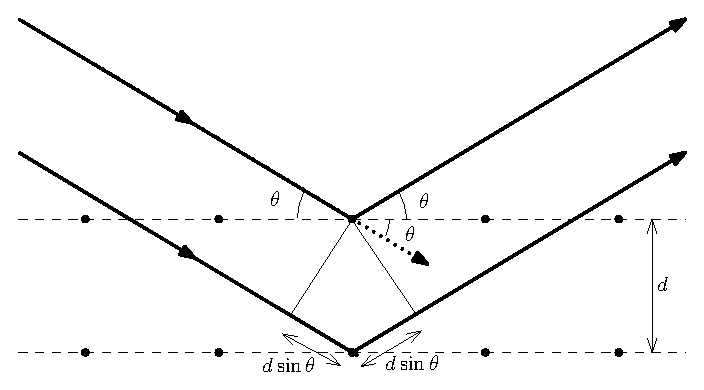
\includegraphics[scale=0.8]{./bragg.eps}
        \caption{Elastic scattering, the Bragg condition.}
        \label{fig:bragg}
        \end{figure}

        Note that the incoming wave suffers a net deviation of $2\theta$.
        Thus, if a beam is targeted at a crystal sample, this particular set of scattered waves form a cone, with cone angle $2\theta$.
        If it strikes a screen at a distance $L$ away, we observe a ring of diameter $D = 2L\tan{2\theta}$.

        In this experiment, we observe Debye-Scherrer diffraction which employs a polycrystalline graphite lattice. This hexagonal lattice
        has two lattice constants, $d_1$ and $d_2$ which lead to the formation of two bright rings of diameters $D_1$ and $D_2$.
        
        \begin{figure}[H]
        \centering
        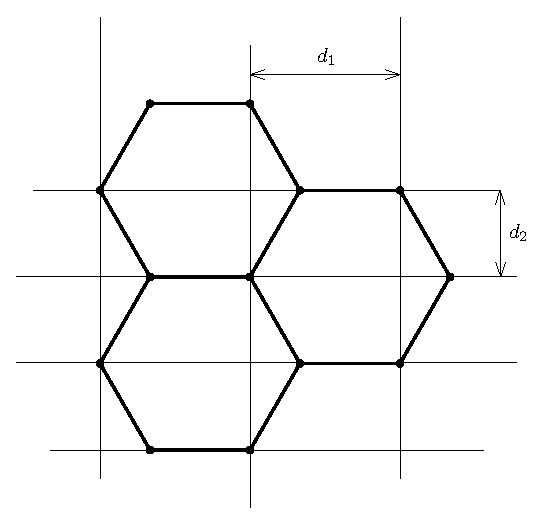
\includegraphics[scale=0.8]{./graphite.eps}
        \caption{Lattice plane spacings in graphite.}
        \label{fig:graphite}
        \end{figure}

        Our electron beam is generated by accelerating electrons emitted from a cathode over a potential $U$. This imparts them with a kinetic
        energy of $eU = p^2 /2m$, which means that they obtain a momentum $p = \sqrt{2mK} = \sqrt{2meU}$. 
        Here, $e$ is the standard electronic charge and $m$ is the mass of the electron.
        Thus, we expect this beam to have a de Broglie wavelength
        \[
                \lambda = \frac{h}{\sqrt{2meU}}.
        \]
        After striking the graphite foil and undergoing diffraction, the brightest rings appear on the screen when $2d\sin\theta = \lambda$.
        For small angles, we approximate $\tan{2\theta} \approx 2\sin\theta \approx 2\theta$, so we obtain
        \[
                \lambda = \frac{dD}{2L}.
        \]
        Comparing these two expressions, we expect
        \[
                D = \frac{2Lh}{d\sqrt{2meU}} = \frac{k}{\sqrt{U}}.
        \]
        Thus, the diameter of the ring is inversely proportional to the square root of the accelerating potential.

        \section{Experimental setup}
        In an electron diffraction tube, a beam of electrons is accelerated by a potential $U$ and targeted on a graphite foil.
        The diffracted beam is allowed to fall on a fluorescent screen on the far end of the tube, from which the diameters of the
        circular maxima are observed. The distance from the graphite foil and the screen is also noted.
        This data is used to deduce the two major lattice spacings of graphite, by plotting $D_i$ versus $1 /\sqrt{U}$
        for each of the rings to obtain the slopes $k_i$. The lattice constant $d_i$ is calculated as
        \[
                d_i = \frac{2Lh}{k_i\sqrt{2me}}.
        \]

        \section{Experimental data and analysis}
        \subsection{Processing and plotting}
        The distance between the graphite and the screen has been measured as $L = 135$ mm.
        The ring diameters have been measured for voltages between $3$ and $5$ kV, three times for each. These three sets of data
        have been presented below.
        \begin{table}[H]
                \centering
                \caption{Diameters of the rings for each accelerating voltage.}
                \label{tab:diameters}
                \begin{tabular}{c|c|c}\hline
                Voltage $U$ (kV)        & $D_1$ (cm)    &  $D_2$ (cm)          \\\hline\hline
                                        & 2.905         &  5.110               \\
                3.0                     & 2.830         &  4.995               \\
                                        & 2.870         &  4.970               \\\hline
                                        & 2.765         &  4.780               \\
                3.5                     & 2.560         &  4.640               \\
                                        & 2.650         &  4.550               \\\hline
                                        & 2.585         &  4.375               \\
                4.0                     & 2.520         &  4.490               \\
                                        & 2.340         &  4.320               \\\hline
                                        & 2.515         &  4.200               \\
                4.5                     & 2.510         &  4.225               \\
                                        & 2.300         &  3.920               \\\hline
                                        & 2.310         &  3.995               \\
                5.0                     & 2.270         &  4.035               \\
                                        & 2.160         &  3.790               \\\hline
                \end{tabular}
        \end{table}
        We plot $D$ vs $1 /\sqrt{U}$ for both $D_1$ and $D_2$ and fit the data linearly. We record the slopes of the fits as $k_1$ and $k_2$.
        \begin{figure}[H]
        \centering
        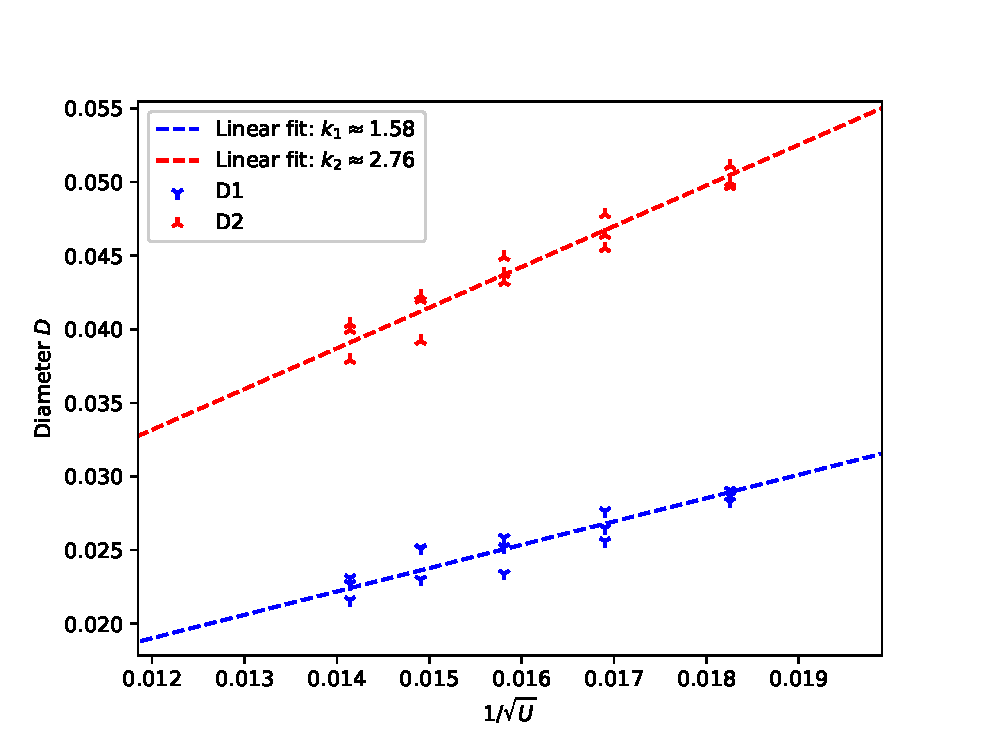
\includegraphics[scale=1.0]{./linear_fit.eps}
        \caption{Data points fitted (least square) to a straight line through the origin.}
        \label{fig:fit}
        \end{figure}

        We obtain
        \[
                k_1 = 1.585, \qquad k_2 = 2.765.
        \]
        The lattice constants $d_1$ and $d_2$ are calculated as
        \[
                d_i = \frac{2Lh}{k_i\sqrt{2me}}.
        \]
        Thus,
        \[
                d_1 = 2.089 \times 10^{-10}\text{ m}, \qquad d_2 = 1.198 \times 10^{-10}\text{ m}.
        \]

        We now calculate $\lambda_i = d_i D / 2L$, and $\lambda_{i,\text{theory}} = h /\sqrt{2 m e U}$.
        \begin{table}[H]
                \centering
                \caption{Diameters and corresponding wavelengths for the first ring.}
                \label{tab:ring_1}
                \begin{tabular}{c|c|c|c|c}\hline
                Voltage $U$ (kV) & $D_1$ (cm)    & $\lambda_1$ (pm)& $\bar{\lambda_1}$ (pm) &$\lambda_{1,\text{theory}}$ (pm) \\\hline\hline
                                 & 2.905         &  22.472         &                    &           \\
                3.0              & 2.830         &  21.892         & 22.189 $\pm$ 0.29  &  22.391   \\
                                 & 2.870         &  22.202         &                    &           \\\hline
                                 & 2.765         &  21.389         &                    &           \\
                3.5              & 2.560         &  19.803         & 20.564 $\pm$ 0.79  &  20.730   \\
                                 & 2.650         &  20.500         &                    &           \\\hline
                                 & 2.585         &  19.997         &                    &           \\
                4.0              & 2.520         &  19.494         & 19.198 $\pm$ 0.98  &  19.391   \\
                                 & 2.340         &  18.102         &                    &           \\\hline
                                 & 2.515         &  19.455         &                    &           \\
                4.5              & 2.510         &  19.417         & 18.888 $\pm$ 0.95  &  18.282   \\
                                 & 2.300         &  17.792         &                    &           \\\hline
                                 & 2.310         &  17.870         &                    &           \\
                5.0              & 2.270         &  17.560         & 17.380 $\pm$ 0.60  &  17.344   \\
                                 & 2.160         &  16.709         &                    &           \\\hline
                \end{tabular}
        \end{table}
        \begin{table}[H]
                \centering
                \caption{Diameters and corresponding wavelengths for the second ring.}
                \label{tab:ring_2}
                \begin{tabular}{c|c|c|c|c}\hline
                Voltage $U$ (kV) & $D_2$ (cm)    & $\lambda_2$ (pm)& $\bar{\lambda_2}$ (pm) &$\lambda_{2,\text{theory}}$ (pm) \\\hline\hline
                                 & 5.110         &  22.677         &                    &           \\
                3.0              & 4.995         &  22.156         & 22.293 $\pm$ 0.34  & 22.391    \\
                                 & 4.970         &  22.046         &                    &           \\\hline
                                 & 4.780         &  21.208         &                    &           \\
                3.5              & 4.640         &  20.582         & 20.658 $\pm$ 0.52  & 20.730    \\
                                 & 4.550         &  20.183         &                    &           \\\hline
                                 & 4.375         &  19.406         &                    &           \\
                4.0              & 4.490         &  19.916         & 19.495 $\pm$ 0.39  & 19.391    \\
                                 & 4.320         &  19.162         &                    &           \\\hline
                                 & 4.200         &  18.630         &                    &           \\
                4.5              & 4.225         &  18.741         & 18.253 $\pm$ 0.75  & 18.282    \\
                                 & 3.920         &  17.388         &                    &           \\\hline
                                 & 3.995         &  17.721         &                    &           \\
                5.0              & 4.035         &  17.898         & 17.477 $\pm$ 0.58  & 17.344    \\
                                 & 3.790         &  16.811         &                    &           \\\hline
                \end{tabular}
        \end{table}
        The following code has been used for the entire process of plotting, fitting and calculation.
        \lstinputlisting[language=Python]{plot.py}
        
        \subsection{Error Analysis}
        We can compare our calculated values for $d_1$ and $d_2$ against literature values.
        \begin{table}[H]
                \centering
                \caption{Parameters and standard/literature values.}
                \label{tab:parameters}
                \begin{tabular}{c|c|c} \hline
                Parameter       & Value                         & Unit  \\\hline\hline
                $d_1$           & $2.13 \times 10^{-10}$        & m     \\
                $d_2$           & $1.23 \times 10^{-10}$        & m     \\
                $m$             & $9.1091 \times 10^{-31}$      & kg    \\
                $e$             & $1.6021 \times 10^{-19}$      & C     \\
                $h$             & $6.6256 \times 10^{-34}$      & J s   \\\hline
                \end{tabular}
        \end{table}
        The deviations from literature values are
        \[
                \Delta d_1 = -0.041 \times 10^{-10}\text{ m}, \qquad \Delta d_2 = -0.032 \times 10^{-10}\text{ m}.
        \]
        The percentage errors are $-1.9\%$ and $-2.6\%$ respectively.

        \subsection{Reported Values}
        We report
        \begin{align*}
                d_1 &= 2.09 \times 10^{-10}\text{ m}, \quad \text{Error: } -1.9\%, \\
                d_2 &= 1.20 \times 10^{-10}\text{ m}, \quad \text{Error: } -2.6\%.
        \end{align*}

        \section{Discussion}
        We see from Tables \ref{tab:ring_1} and \ref{tab:ring_2} that the calculated wavelengths agree well with the theoretical values,
        within one standard deviation. This is in accordance with the de Broglie equation.

        We note that with prior knowledge of the lattice constants, this method could be instead used to determine Planck's constant to
        a reasonable level of accuracy.

        This particular technique is commonly used in the field of X-ray crystallography, in order to obtain the molecular structure
        of crystals. There is a particularly nice interpretation of scattering in terms of Fourier transforms -- if the 
        electronic density in the crystal is $f(\bvec{r})$, diffraction gives us information about its Fourier transform $F(\bvec{g})$,
        where the vectors $\bvec{g}$ are part of the reciprocal or Fourier space.
        
        \subsection{Sources of error}
        The most significant source of error is introduced by the diameter measurements, which have uncertainties of up to 2 mm.
        This is reflected in the wide range in values in $D_i$ for a given $U$, as seen in Table \ref{tab:diameters}.
        Further systematic errors may arise from improper calibration of the electron gun, improper centering of the beam or even 
        a slight tilt in the screen from the perpendicular which would distort the shape of the ring into an ellipse.
        
        \section{Conclusion}
        In conclusion, we have observed the phenomenon of electron diffraction and used this to verify de Broglie's equation,
        thus experimentally demonstrating wave-particle duality. We have further determined the lattice plane spacing constants of graphite
        with errors of less than $3\%$.

        % \nocite{*}
        % \bibliographystyle{plain}
        % \bibliography{ref}

\end{document}
